\documentclass[modern]{aastex62}

\usepackage{units}

\newcommand{\MESA}{{\tt MESA}}

% define some useful commands
\newcommand{\Msun}{\ensuremath{\mathrm{M}_\odot}}
\newcommand{\gcc}{\ensuremath{\mathrm{g\,cm^{-3}}}} % density units

\newcommand{\Mch}{\ensuremath{\mathrm{M}_{\rm Ch}}}

\newcommand{\Ye}{\ensuremath{Y_{\rm e}}}
\newcommand{\EF}{\ensuremath{E_{\rm F}}}

% central quantities
\newcommand{\Tc}{\ensuremath{T_{\rm c}}}
\newcommand{\Rhoc}{\ensuremath{\rho_{\rm c}}}

\newcommand{\epsnu}{\ensuremath{\epsilon_{\nu}}} % Neutrino loss rate
\newcommand{\epsnuc}{\ensuremath{\epsilon_{\mathrm{nuc}}}} % Neutrino loss rate


% nuclides.tex
% input file with macros for nuclides

% base command
\newcommand{\nuclei}[2]{\ensuremath{\mathrm{^{#1}#2}}}

% nuclides, with most highest abundance or longest half-life as default
% for example, \carbon produces ^{12}C, \carbon[13] produces ^{13}C
%
\newcommand{\hydrogen}[1][1]{\nuclei{#1}{H}}
\newcommand{\helium}[1][4]{\nuclei{#1}{He}}
\newcommand{\lithium}[1][7]{\nuclei{#1}{Li}}
\newcommand{\beryllium}[1][9]{\nuclei{#1}{Be}}
\newcommand{\boron}[1][11]{\nuclei{#1}{B}}
\newcommand{\carbon}[1][12]{\nuclei{#1}{C}}
\newcommand{\nitrogen}[1][14]{\nuclei{#1}{N}}
\newcommand{\oxygen}[1][16]{\nuclei{#1}{O}}
\newcommand{\fluorine}[1][19]{\nuclei{#1}{F}}
\newcommand{\neon}[1][20]{\nuclei{#1}{Ne}}
\newcommand{\sodium}[1][23]{\nuclei{#1}{Na}}
\newcommand{\magnesium}[1][24]{\nuclei{#1}{Mg}}
\newcommand{\aluminum}[1][27]{\nuclei{#1}{Al}}
\newcommand{\silicon}[1][28]{\nuclei{#1}{Si}}
\newcommand{\phosphorus}[1][31]{\nuclei{#1}{P}}
\newcommand{\sulfur}[1][32]{\nuclei{#1}{S}}
\newcommand{\chlorine}[1][35]{\nuclei{#1}{Cl}}
\newcommand{\argon}[1][36]{\nuclei{#1}{Ar}}
\newcommand{\potassium}[1][39]{\nuclei{#1}{K}}
\newcommand{\calcium}[1][40]{\nuclei{#1}{Ca}}
\newcommand{\scandium}[1][45]{\nuclei{#1}{Sc}}
\newcommand{\titanium}[1][48]{\nuclei{#1}{Ti}}
\newcommand{\vanadium}[1][51]{\nuclei{#1}{V}}
\newcommand{\chromium}[1][52]{\nuclei{#1}{Cr}}
\newcommand{\manganese}[1][55]{\nuclei{#1}{Mn}}
\newcommand{\iron}[1][56]{\nuclei{#1}{Fe}}
\newcommand{\cobalt}[1][59]{\nuclei{#1}{Co}}
\newcommand{\nickel}[1][58]{\nuclei{#1}{Ni}}
\newcommand{\copper}[1][63]{\nuclei{#1}{Cu}}
\newcommand{\zinc}[1][64]{\nuclei{#1}{Zn}}
\newcommand{\gallium}[1][69]{\nuclei{#1}{Ga}}
\newcommand{\germanium}[1][74]{\nuclei{#1}{Ge}}
\newcommand{\arsenic}[1][75]{\nuclei{#1}{As}}
\newcommand{\selenium}[1][80]{\nuclei{#1}{Se}}
\newcommand{\bromine}[1][79]{\nuclei{#1}{Br}}
\newcommand{\krypton}[1][84]{\nuclei{#1}{Kr}}
\newcommand{\rubidium}[1][85]{\nuclei{#1}{Rb}}
\newcommand{\strontium}[1][88]{\nuclei{#1}{Sr}}
\newcommand{\yttrium}[1][89]{\nuclei{#1}{Y}}
\newcommand{\zirconium}[1][94]{\nuclei{#1}{Zr}}
\newcommand{\niobium}[1][93]{\nuclei{#1}{Nb}}
\newcommand{\molybdenum}[1][98]{\nuclei{#1}{Mo}}
\newcommand{\technetium}[1][97]{\nuclei{#1}{Tc}}
\newcommand{\ruthenium}[1][102]{\nuclei{#1}{Ru}}
\newcommand{\rhodium}[1][103]{\nuclei{#1}{Rh }}
\newcommand{\palladium}[1][106]{\nuclei{#1}{Pd}}
\newcommand{\silver}[1][107]{\nuclei{#1}{Ag}}
\newcommand{\cadmium}[1][114]{\nuclei{#1}{Cd}}
\newcommand{\indium}[1][115]{\nuclei{#1}{In}}
\newcommand{\tin}[1][120]{\nuclei{#1}{Sn}}
\newcommand{\antimony}[1][121]{\nuclei{#1}{Sb}}
\newcommand{\tellurium}[1][130]{\nuclei{#1}{Te}}
\newcommand{\iodine}[1][127]{\nuclei{#1}{I}}
\newcommand{\xenon}[1][132]{\nuclei{#1}{Xe}}
\newcommand{\cesium}[1][133]{\nuclei{#1}{Cs}}
\newcommand{\barium}[1][138]{\nuclei{#1}{Ba}}
\newcommand{\lanthanum}[1][139]{\nuclei{#1}{La}}
\newcommand{\cerium}[1][140]{\nuclei{#1}{Ce}}
\newcommand{\praseodymium}[1][141]{\nuclei{#1}{Pr}}
\newcommand{\neodymium}[1][142]{\nuclei{#1}{Nd}}
\newcommand{\promethium}[1][147]{\nuclei{#1}{Pm}}
\newcommand{\samarium}[1][152]{\nuclei{#1}{Sm}}
\newcommand{\europium}[1][153]{\nuclei{#1}{Eu}}
\newcommand{\gadolinium}[1][158]{\nuclei{#1}{Gd}}
\newcommand{\terbium}[1][159]{\nuclei{#1}{Tb}}
\newcommand{\dysprosium}[1][164]{\nuclei{#1}{Dy}}
\newcommand{\holmium}[1][165]{\nuclei{#1}{Ho}}
\newcommand{\erbium}[1][168]{\nuclei{#1}{Er}}
\newcommand{\thulium}[1][169]{\nuclei{#1}{Tm}}
\newcommand{\ytterbium}[1][174]{\nuclei{#1}{Yb}}
\newcommand{\lutetium}[1][175]{\nuclei{#1}{Lu}}
\newcommand{\hafnium}[1][180]{\nuclei{#1}{Hf}}
\newcommand{\tantalum}[1][180]{\nuclei{#1}{Ta}}
\newcommand{\tungsten}[1][184]{\nuclei{#1}{W}}
\newcommand{\rhenium}[1][187]{\nuclei{#1}{Re}}
\newcommand{\osmium}[1][192]{\nuclei{#1}{Os}}
\newcommand{\iridium}[1][193]{\nuclei{#1}{Ir}}
\newcommand{\platnium}[1][195]{\nuclei{#1}{Pt}}
\newcommand{\gold}[1][197]{\nuclei{#1}{Au}}
%\newcommand{\mercury}[1][202]{\nuclei{#1}{Hg}}
\newcommand{\thallium}[1][205]{\nuclei{#1}{Tl}}
\newcommand{\lead}[1][208]{\nuclei{#1}{Pb}}
\newcommand{\bisumth}[1][209]{\nuclei{#1}{Bi}}
\newcommand{\polonium}[1][208]{\nuclei{#1}{Po}}
\newcommand{\astatine}[1][219]{\nuclei{#1}{At}}
\newcommand{\radon}[1][222]{\nuclei{#1}{Rn}}
\newcommand{\francium}[1][223]{\nuclei{#1}{Fr}}
\newcommand{\radium}[1][226]{\nuclei{#1}{Ra}}
\newcommand{\actinium}[1][227]{\nuclei{#1}{Ac}}
\newcommand{\thorium}[1][232]{\nuclei{#1}{Th}}
\newcommand{\protactinium}[1][231]{\nuclei{#1}{Pa}}
\newcommand{\uranium}[1][238]{\nuclei{#1}{U}}
\newcommand{\neptunium}[1][237]{\nuclei{#1}{Np}}
\newcommand{\plutonium}[1][244]{\nuclei{#1}{Pu}}
\newcommand{\americium}[1][243]{\nuclei{#1}{Am}}
\newcommand{\curium}[1][248]{\nuclei{#1}{Cm}}
\newcommand{\berkelium}[1][247]{\nuclei{#1}{Bk}}
\newcommand{\californium}[1][251]{\nuclei{#1}{Cf}}
\newcommand{\einsteinium}[1][252]{\nuclei{#1}{Es}}
\newcommand{\fermium}[1][257]{\nuclei{#1}{Fm}}
\newcommand{\mendelevium}[1][260]{\nuclei{#1}{Md}}
\newcommand{\nobelium}[1][259]{\nuclei{#1}{No}}
\newcommand{\lawrencium}[1][262]{\nuclei{#1}{Lr}}
\newcommand{\rutherfordium}[1][261]{\nuclei{#1}{Rf}}
\newcommand{\dubnium}[1][262]{\nuclei{#1}{Db}}
\newcommand{\seaborgium}[1][266]{\nuclei{#1}{Sg}}
\newcommand{\bohrium}[1][267]{\nuclei{#1}{Bh}}
\newcommand{\hassium}[1][269]{\nuclei{#1}{Hs}}
\newcommand{\meitnerium}[1][268]{\nuclei{#1}{Mt}}
\newcommand{\darmstadtium}[1][271]{\nuclei{#1}{Ds}}


\usepackage{amsmath}

\begin{document}

% \author[0000-0002-4870-8855]{Josiah Schwab}
% \altaffiliation{Hubble Fellow}
% \affiliation{Department of Astronomy and Astrophysics, University of California, Santa Cruz, CA 95064, USA}
% \correspondingauthor{Josiah Schwab}
% \email{jwschwab@ucsc.edu}

% \title{}

\section{Relevant Timescales}

We define the accretion timescale as
\begin{equation}
  t_{\mathrm{accrete}} = \frac{M}{\dot{M}}
\end{equation}
and the compression timescale as
\begin{equation}
  \label{eq:tcompress}
  t_{\mathrm{compress}} = \left(\frac{d \ln \rho}{dt} \right)^{-1}~.
\end{equation}
The central density rises rapidly as one approaches the Chandrasekhar
mass and therefore the compression timescale is significantly shorter
than the accretion timescale (by a factor $\sim 100$).


We define the electron-capture timescale as
\begin{equation}
  \label{eq:tcapture}
  t_{\mathrm{capture}} = \left(\frac{d \ln \Ye}{dt} \right)^{-1}
\end{equation}
and the heating timescale as
\begin{equation}
  \label{eq:cooling}
  t_{\mathrm{heat}} = \frac{c_P T}{\epsnuc} ~.
\end{equation}
We will primarily be interested in the exothermic electron captures,
but we will plot the absolute value of this quantity so that it
represents the cooling timescale at times when the Urca-process is
operating.


For the plots of these timescales in previous work on ECSN
progenitors, see Figure 7 in \citet{Miyaji1980}, Figure 2 in
\citet{Miyaji1987}, and Figure 9 in \citet{Takahashi2013}.

The figures show these timescales for for an ONe WD accreting at
$\dot{M} = 10^{-6}\,\Msunyr$.  Two WD models are shown: SQB15 is the
fiducial model used in \citet{Schwab2015}, which has only even-A
isotopes (\oxygen[16], \neon[20], \magnesium[24]); SBQ17 is the
fiducial model used in \citet{Schwab2017a}, which also includes the
odd-A isotopes \sodium[23] and \magnesium[25] and experiences
significant Urca-process cooling.  Table 1 gives the detailed
compositions.  We show a run using the ``on-the-fly'' rates in \MESA\
assuming only allowed transitions contribute and another run assuming
the non-unique second forbidden transitions have
$\log(ft) \approx 11$.  We also show the results of using the
\citet{Suzuki2016a} tables.  In these tables, the relevant non-unique
second forbidden transition for \neon[20] is at the (previous)
experimental upper limit.

The models in Figure 3 all want to convect around the time of the
$A=24$ electron captures, but in these runs we have artificially
suppressed convection.  (Once the models become convective in this
regime, \MESA\ struggles for a variety of reasons.)

The \MESA\ models all halt at oxygen ignition.  The heating/capture
timescales will naturally continue to decrease beyond this point.


\begin{table}
  \centering
  \caption{The set of compositions used in our \MESA\ models.  Each
    composition is referenced in the text by the identifier listed in
    the top row.  Each column lists the mass fractions of the isotopes
    (listed at left) that were included.  Dashes indicate that a
    particular isotope was not included.}
  \label{tab:compositions}
  \begin{tabular}{rcc}
    \hline
    Isotope & SQB15 & SBQ17 \\
    \hline
    \oxygen[16]    & 0.500 & 0.500 \\
    \neon[20]      & 0.450 & 0.390 \\
    \neon[22]      & ---   & ---   \\
    \sodium[23]    & ---   & 0.050 \\
    \magnesium[24] & 0.050 & 0.050 \\
    \magnesium[25] & ---   & 0.010 \\
    \hline
  \end{tabular}
\end{table}

\begin{figure}
  \centering
  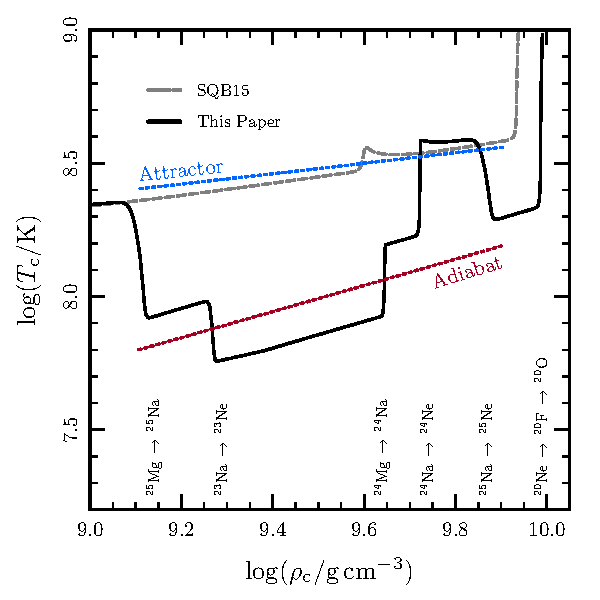
\includegraphics[width=\textwidth]{schematic.pdf}
  \caption{Central density-temperature evolution for of the accreting
    WD models with the effects of various reactions labeled. (This is
    Figure 5 in \citealt{Schwab2017a}.)}
\end{figure}


\bibliography{timescales.bib}

\begin{figure}
  \centering
  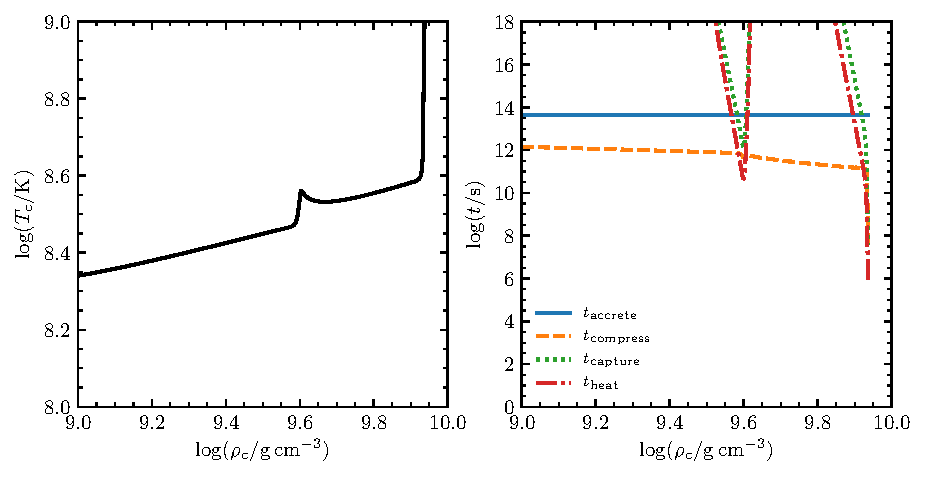
\includegraphics[width=\textwidth]{SQB15-allowed.pdf}
  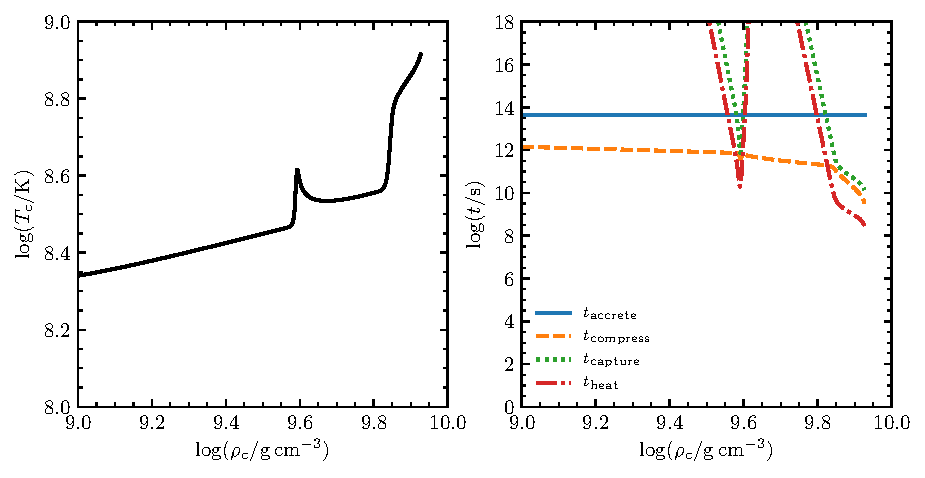
\includegraphics[width=\textwidth]{SQB15-nusf11.pdf}
    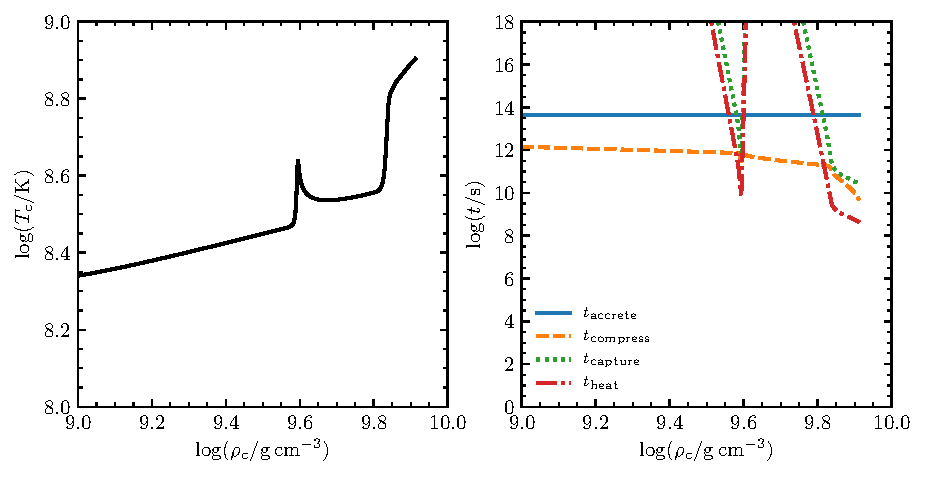
\includegraphics[width=\textwidth]{SQB15-suzuki.pdf}
  \caption{Evolution without Urca-process cooling (SQB15 model).  \textit{Upper panel}: On-the-fly rates with allowed transitions only;  \textit{Middle panel}: On-the-fly rates including non-unique second forbidden transitions; \textit{Lower panel}: \citet{Suzuki2016a} rate tables.}
\end{figure}

\begin{figure}
  \centering
  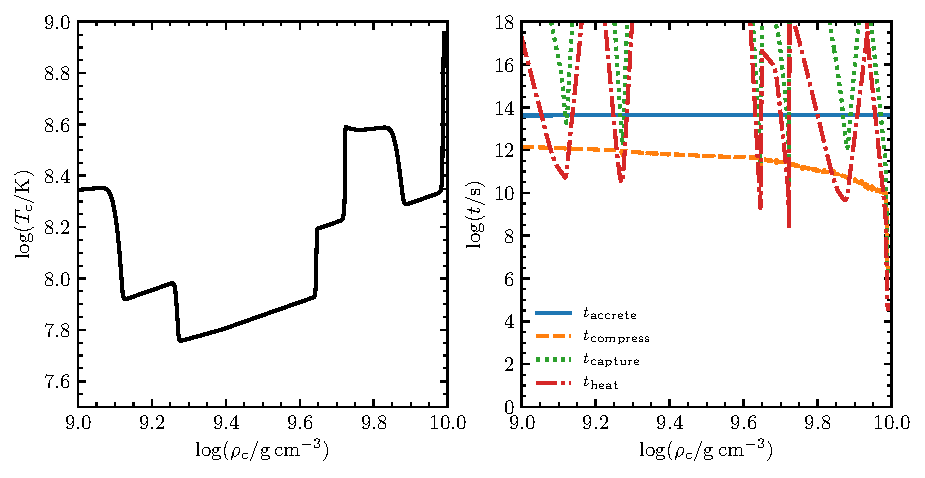
\includegraphics[width=\textwidth]{SBQ17-allowed.pdf}
  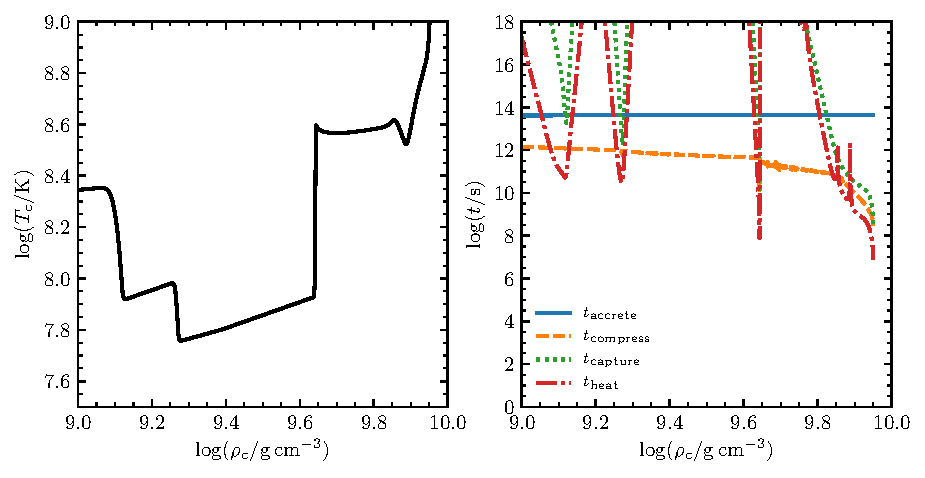
\includegraphics[width=\textwidth]{SBQ17-nusf11.pdf}
  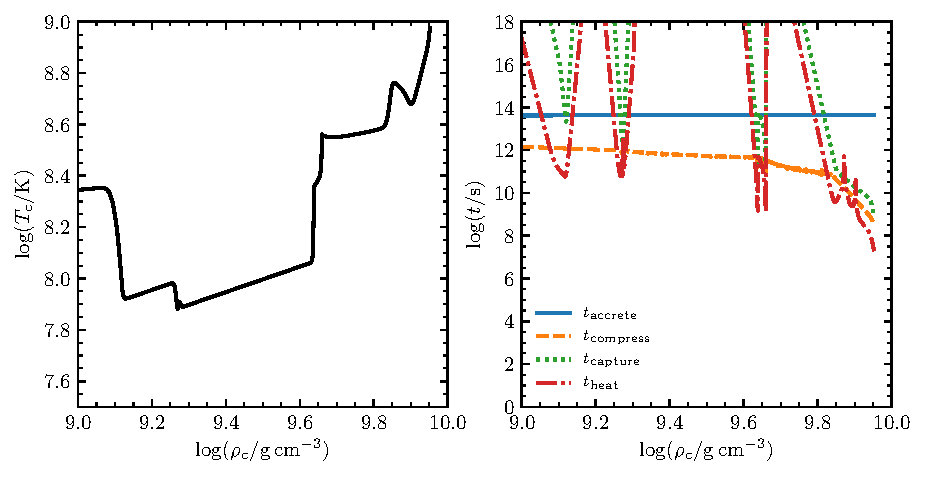
\includegraphics[width=\textwidth]{SBQ17-suzuki.pdf}
  \caption{Evolution with Urca-process cooling (SBQ17 model). \textit{Upper panel}: On-the-fly rates with allowed transitions only;  \textit{Middle panel}: On-the-fly rates including non-unique second forbidden transitions; \textit{Lower panel}: \citet{Suzuki2016a} rate tables.}
\end{figure}






\end{document}

%%% Local Variables:
%%% mode: latex
%%% TeX-master: t
%%% End:
